% ---------------------------------------------------------------
% ---------------------------------------------------------------
% This template was developed for the working paper series of 
% the Interdisciplinary Laboratory of Computational Social Science (iLCSS)
% at the University of Maryland, College Park

% The template was built based on  the PNAS Latex model. 

% Adjustments were made by Tiago Ventura, Ph.D. Student in Political Science at UMD, 
% and researcher at the iLCSS.

\documentclass[9pt,twocolumn,twoside]{ilcss}




\templatetype{ilcssworkingpaper} % Choose template 

\title{\ M\'etodos de aprendizaje de \'maquina para inferir el nivel de cobertura de banda ancha fija en municipios  de M\'exico}	

% Use letters for affiliations, numbers to show equal authorship (if applicable) and to indicate the corresponding author
\author[a]{C\'esar Zamora Mart\'inez}
%\author[b,1,2]{Author Two} 
%\author[a]{Author Three}

\affil[a]{Alumno de Maestr\'ia en Ciencias de Datos (ITAM)}
%\affil[b]{Affiliation Two}
%\affil[c]{Affiliation Three}

% Please give the surname of the lead author for the running footer
\leadauthor{C\'esar Zamora Mart\'inez} 

% Please add here a significance statement to explain the relevance of your work
%\significancestatement{Authors must submit a 120-word maximum statement about the significance of their research paper written at a level understandable to an undergraduate educated scientist outside their field of speciality. The primary goal of the Significance Statement is to explain the relevance of the work in broad context to a broad readership. The Significance Statement appears in the paper itself and is required for all research papers.}

% Please include corresponding author, author contribution and author declaration information
%\authorcontributions{Please provide details of author contributions here.}
%\authordeclaration{Please declare any conflict of interest here.}
%\equalauthors{\textsuperscript{1}A.O.(Author One) and A.T. (Author Two) contributed equally to this work (remove if not applicable).}
\correspondingauthor{\textsuperscript{2}E-mail: czamora5\@email.itam.mx}

% Keywords are not mandatory, but authors are strongly encouraged to provide them. If provided, please include two to five keywords, separated by the pipe symbol, e.g:
%\keywords{Aprendizaje de Máquina $|$ Banda Ancha $|$ Telecomunicaciones $|$ ITAM} 

\begin{abstract}Aunque en fechas recientes se reconoce el impacto benéfico que la banda ancha tienen sobre en entorno económico y social, la penetración de tales servicios en los municipios obedece a múltiples factores que inciden en el despliegue de la infraestructura que permite su prestación. Motivado por ello, en este trabajo se plantea el uso de métodos basados en aprendizaje de máquina que permitan clasificar los municipios conforme a su nivel de  cobertura a través de indicadores de penetración y establecer factores que propician o desincentivan los despliegues de banda ancha fija.
\end{abstract}

%\dates{This manuscript was compiled on \today}

% You can change the link on the footer here

%\doi{\url{http://ilcss.umd.edu/}}

\begin{document}

\maketitle
\thispagestyle{firststyle}
\ifthenelse{\boolean{shortarticle}}{\ifthenelse{\boolean{singlecolumn}}{\abscontentformatted}{\abscontent}}{}

% If your first paragraph (i.e. with the \dropcap) contains a list environment (quote, quotation, theorem, definition, enumerate, itemize...), the line after the list may have some extra indentation. If this is the case, add \parshape=0 to the end of the list environment.

\dropcap{D}urante las últimas tres décadas las telecomunicaciones han tenido un avance sin precedentes en el mundo, posicionándose como herramientas que potencian el desarrollo económico y social, pues, como ha sido ampliamente documentado en la literatura (\cite{PRADHAN2014634}), permiten crear oportunidades, reducir la pobreza e impulsar el progreso económico y social para el bienestar de la población\footnote{\cite{Katz2018} muestra que un avance del 1\% en un índice sobre digitalización, genera un incremento de la productividad que redunda en un crecimiento económico de un 0.3\% del PIB. }. Uno de los ejes que permiten explicar lo anterior es el impacto benéfico de los servicios de banda ancha en los procesos productivos, financieros y en general el bienestar de la población (\cite{Katz2012}).

En México, a cerca de cuatro años de la reforma a de telecomunicaciones en 2013, que llevo a la promulgación de la Ley Federal de Telecomunicaciones y Radiodifusión (LFTyR) junto con la creación del Instituto Federal de Telecomunicaciones (IFT), se estimó un crecimiento superior al 37\% en las conexiones de banda ancha fija (BAF), traduciéndose a que para entonces casi la mitad los hogares contaban con servicios de Internet (\cite{IFT2017} e \cite{IFT2018}).

Aunque este fenómeno revela una tendencia favorable con respecto al entorno internacional\footnote{A finales de 2018 México fue el cuarto país con mayor crecimiento de penetración de banda ancha fija entre los países de la Organización para la Cooperación y Desarrollo Económicos (OCDE); y mostró un crecimiento de 17.9\% en la penetración de accesos por medio de fibra óptica (\cite{IFT2019})}, la Encuesta sobre Disponibilidad y Uso de Tecnologías de la Información y la Comunicación en los Hogares 2018 (ENDUTIH 2018, \cite{ENDUTIH2018}) dejó en claro la existencia de una brecha en la adopción de estos servicios para la población mexicana (por tanto en sus conducentes beneficios), pues sólo cerca de 65.8\% de la población con seis años o más es usuario de servicios de Internet en los hogares del país, además de que mostró que este es un fenómeno urbano, puesto el 73.1\% del total de la población urbana son usuarios de este servicio en contraste con la población conectada en zonas rurales que es cercana a 40.6\%.

A efecto de explicar el entorno de la penetración de servicios de Internet a nivel municipal, en adelante nos centraremos en los servicios de banda ancha fija\footnote{Ello dado que desafortunadamente, el Banco de Información de Telecomunicaciones (BIT) del IFT sólo posee el detalle desagregado de servicios de Internet de banda ancha móvil para nivel estado, sin que se hayan podido localizar fuentes con datos precisos al respecto.}, los cuales son servicios de acceso a Internet y transmisión de datos orientados a usuarios finales (personas físicas o empresas), que se brindan a través de equipos terminales (módems, terminales ópticas y demás) que tienen una ubicación geográfica determinada y fija (\cite{IFT2018man}). Ello obliga a los operadores de telecomunicaciones interesados a realizar inversiones que les permitan alcanzar los puntos geográficos en donde se localizan los clientes potenciales, esto es, cerca de hogares y edificios de empresas, aprovechando las capacidades de las tecnologías en las que se basan sus redes. 

Dicho contexto les condiciona a establecer un circuito físico o virtual a través del cual se pueda conectar la ubicación del usuario a la red del operador y a través del que se prestarán los servicios (“Acceso de datos” o simplemente como “acceso”, \cite{IFT2018man}). Por ende, dado que afrontan costos considerables en infraestructura, equipos, permisos y recursos humanos para poder brindar servicios\footnote{En línea con \cite{IFT2017reb}, no sólo se enfrentan costos directos, sino oportunidad y de transacción; así como el riesgo de afrontar costos hundidos.}, típicamente los operadores concentran su oferta en zonas densamente pobladas donde existe suficiente capacidad económica para asegurar no solo que recuperarán sus inversiones sino que serán rentables desde la visión de negocio.

%Además de los aspectos socio-económicos, también se destacan otros factores que pueden ser tomados en cuentan por un operador para evaluar una zona como idónea para brindar servicios: 1) Viabilidad de permisos para desarrollar los despliegues (e.g. concesiones para operar, medio ambiente), 2) viabilidad tecnológica (e.g. limitadas técnicas por la distancia que limitan la velocidad, calidad, entre otras), 3) existencia de infraestructura cercana a la zona de la que puedan disponer para proveer servicios (por ejemplo, propia o arrendada); y 4) existencia de competencia en el área; es decir de proveedores de servicios de telecomunicaciones.
%	
%Por otro lado, un indicador ampliamente usado en el sector de telecomunicaciones (\cite{Hanafizadeh},\cite{IFT2017reb},\cite{IFT2018man}) para cuantificar la cobertura de banda ancha fija es medir la penetración en una zona con la cantidad de accesos en ella por cada 100 hogares:
%\begin{equation}\label{pen_hogares}
%PenBAFHogares = \frac{Accesos }{Hogares} \times 100 
%\end{equation}
%
%Este indicador tiene las siguientes limitaciones 1) la presencia de accesos en un municipio no implica necesariamente que las localidades que lo conforman cuentan con infraestructura para brindar estos servicios \footnote{A guisa de ejemplo, puede ser el caso que únicamente existan servicios de BAF en la cabecera municipal, pero no en el resto de sus comunidades}, 2) la penetración se puede subestimar si no se tienen un división explícita entre accesos de usuarios residenciales y empresariales.
%
%En vista de este último punto, 

Para cuantificar la cobertura de banda ancha fija la OCDE define una medida de penetración en una zona como la cantidad de accesos en ella por cada 100 habitantes, el cual es un proxy del indicador de suscriptores por cada 100 habitantes\footnote{http://www.oecd.org/internet/broadband/broadband-faqs.htm}:
\begin{equation}\label{pen_habitantes}
PenBAFHabitantes = \frac{Accesos }{Habitantes} \times 100 
\end{equation}

En este sentido, de acuerdo a la información publicada por este organismo a diciembre de 2018, sus países miembros contaban con una penetración media de 30.92 accesos por cada 100 habitantes, ocupando México el penúltimo lugar (con 14.83 accesos por cada 100 habitantes).

Por otro lado, para BAF los accesos se basan típicamente en las tecnologías\footnote{También existen configuraciones híbridas} (\cite{moya2014telecomunicaciones}): 1) DSL: tecnología de transmisión por cable trenzado de cobre, su disponibilidad y la velocidad dependen de la distancia; 2) Cable coaxial: se forma por dos hilos de cobre cuya estructura permite permite, en generala más capacidad para transmitir información que el par trenzado de cobre; 3) Fibra óptica: formados por un medio de vidrio o polímero que permite el paso de haces de luz, pueden transmitir más de 10 Gbit/s hasta a 10 kilómetros de distancia, 4) Otras: incluye uso de ondas electromagnéticas como microondas, señales satélites y demás; usualmente  tienen menor desempeño comparado a 1), 2) o 3), pero son viables en regiones de difícil acceso.

Con todo lo anterior, el objetivo del presente documento será plantear un modelo con métodos de aprendizaje de máquina que permitan identificar variables útiles para explicar el nivel de penetración de BAF (por ejemplo, datos geográficos y demográficos) así como de los factores que inciden en los despliegues de tecnologías capaces de dar servicios de Internet de alta velocidad. 

En este sentido, con motivo de estudiar a los municipios que cuentan penetración de BAF basada en tecnologías capaces de dar servicios de velocidad alta, se enfocarán los indicadores de penetración presentados previamente sobre accesos correspondientes a tecnologías de cable coaxial o fibra óptica (es decir, se calcularan con respecto la cantidad de accesos resultado de sumar de los que correspondan a cable coaxial y aquellas de fibra óptica en cada municipio).

\section{Revisión y análisis de fuentes de datos asociados a banda ancha fija}

A continuación se resumen las fuentes de información consultadas con relación a servicios de BAF, junto con las consideraciones particulares derivadas de su exploración\footnote{El procesamiento de la información se llevó a cabo a través de scripts en Bash, R y Python, disponibles en el Anexo A de este documento}. 

\subsection{Revisión de fuentes de información}

En términos generales, la revisión abarcó datos públicos 
de fuentes gubernamentales y organismos internacionales relativos a siguientes los ejes:

\subsubsection{Identificación de municipios}

Dado que la disponibilidad de información social y demográfica en fuentes públicas con desglose municipal se encuentra limitada a ejercicios estadísticos que abarcan hasta el año 2015 (\cite{Intercensal2015}, \cite{CONAPO2015}, \cite{ONU2015}), la identificación de los municipios se hizo de manera congruente el marco metodológico de la Encuesta Intercensal 2015 en donde se contabilizaron un total de 2,457 municipios.

\subsubsection{Datos de accesos de banda ancha}

El Banco de Información de Telecomunicaciones (\cite{IFT2019BIT}) posee datos históricos (de 2013 a mediados 2019) sobre los accesos de banda ancha móvil y fija de México; sin embargo únicamente en el segundo caso se ofrece el detalle a nivel municipio. Dicha fuente provee datos de 29 empresas a las que pertenecen los accesos de BAF junto tecnología correspondiente (DSL, cable coaxial, fibra óptica, satelital y otras), sin proveer el desglose entre accesos residenciales o no residenciales. Se consideró relevante extraer los datos accesos en cada municipio, agregando los datos de todos los operadores por tecnología de acceso para el periodo con información más reciente (junio de 2019).

\subsubsection{Datos socio-económicos}
A través de la Encuesta Intercensal 2015 (\cite{Intercensal2015}), el INEGI reúne información de componentes que describen la evolución de la población, junto con sus viviendas y de sus condiciones socio-económicas.Tras estudiar esta fuente, los datos que se han considerado de interés para el estudio a nivel municipal la penetración de BAF son: 1) número de hogares, 2) número de habitantes, 3) porcentaje de viviendas que cuentan con disponibilidad de servicios de telecomunicaciones (es decir, a través de telefonía fija, telefonía celular, televisión de paga e Internet). 

%Dicha elección se apoya en que, como se ha mencionado previamente, los despliegues de redes fijas se realizan alrededor de donde se ubican los clientes potenciales, y a su vez en el hecho de que la presencia de servicios de telecomunicaciones (incluso distintos a BAF) constituye una señal de que existen condiciones positivas para que los operadores desarrollen una cadena de elementos de infraestructura y operación que le permitan atender en una zona específica ofreciendo servicios a la población.

\subsubsection{Datos asociados a marginación}

La Comisión Nacional de Población (CONAPO) diseño una herramienta denominada "índice de marginación" para realizar mediciones de las carencias que padece la población (\cite{CONAPO2015}). Esta recoge una serie de dimensiones socio-económicas para su construcción: educación, vivienda, y distribución de la población e ingresos. Para explorar la relación de tales ejes con la penetración de servicios de BAF, se consideró relevante involucrar a las siguientes mediciones empleadas por CONAPO en 2015 para la construcción de dicho índice a) porcentaje de ocupantes en viviendas sin energía eléctrica, b) porcentaje de población en localidades con menos de 5,000 habitantes, y c) porcentaje de población ocupada con ingresos de hasta 2 salarios

%\begin{itemize}
	%\item Porcentaje de población de 15 años o más analfabeta,	
	%\item Porcentaje de población de 15 años o más sin primaria completa,	
	%\item Porcentaje de ocupantes en viviendas sin drenaje ni excusado,	
	%\item Porcentaje de ocupantes en viviendas sin energía eléctrica,\vspace{-0.1cm}	
	%\item Porcentaje de ocupantes en viviendas sin agua entubada,	
	%\item Porcentaje de viviendas con algún nivel de hacinamiento,	
	%\item Porcentaje de ocupantes en viviendas con piso de tierra,	
	%\item Porcentaje de población en localidades con menos de 5,000 habitantes,\vspace{-0.3cm}	
	%\item Porcentaje de población ocupada con ingresos de hasta 2 salarios.\vspace{-0.2cm} mínimo.	
%\end{itemize}

%La elección de tales variables se basa en que: a) la energía eléctrica es una condición necesaria para el funcionamiento de los servicios de telecomunicaciones, b) los operadores deben de hacer mayores esfuerzos para atender zonas que son bajamente pobladas donde puede no ser rentable llevar servicios, y c)
 
\subsubsection{Datos asociados a desarrollo humano}

El Programa de las Naciones Unidas para el Desarrollo (PNUD) es una organización orientada a generar soluciones a los países que buscan alcanzar sus metas de desarrollo y lograr los objetivos compartidos con la comunidad internacional. Como parte de sus actividades en México \cite{ONU2015}, periódicamente evalúan el nivel de desarollo de los municipios a través de la construcción del "Índice de Desarrollo Humano (IDH)", el cual considera los ejes de salud, eduación e ingreso. Al respecto, puesto que el ingreso de la población es un componente relevante en el acceso a servicios de telecomunicaciones, se considerarán los datos del PNUD empleados para la estimación del IDH correspondientes al año 2015 relativos el ingreso bruto per cápita en poder de paridad de compra (PPC), expresado en dólares estadounidenses, de cada municipio\footnote{Estos datos no se encuentra disponibles para 11 municipios. 
	%A saber 5 del estado de Chihuahua (Buenaventura, Carichí, Santa Isabel, Temósachic, y Urique), 4 en Oaxaca (Matías Romero Avendaño, Santa María Chimalapa, Santa María Petapa y San Francisco Chindúa), uno en Puebla (San Nicolás de los Ranchos) y otro en Sonora (General Plutarco Elías Calles)
}.

\subsection{Consideraciones sobre la información reunida}

En términos de la información reunida, la exposición previa (así como la metodología propuesta por \cite{IFTcobertura2018}), el análisis de cobertura para servicios de BAF partirá de las siguientes premisas:

\begin{itemize}
	\item \textbf{Periodo de la información de accesos:} junio de 2019,\vspace{-0.2cm}
	\item \textbf{Nivel de desagregación geográfico:} municipal considerando los municipios de la Encuesta Intercensal 2015 (\cite{Intercensal2015}),\vspace{-0.2cm}
	\item \textbf{Indicador de cobertura:} se considerarán dos ejercicios, uno basado en la penetración por cada 100 hogares y otro en penetración por cada 100 habitantes (ver ec. \ref{pen_hogares} y \ref{pen_habitantes}),\vspace{-0.2cm} 
	\item \textbf{Tipo tecnologías de acceso para establecer cobertura:} cable coaxial y fibra óptica, bajo la premisa de que
	pueden ser usadas para proveer servicios con velocidades mayores que otras opciones,\vspace{-0.2cm}
	\item \textbf{Identificación de municipios con cobertura de BAF:} aquellos que son reportados, de manera explícita en el BIT, como con presencia de accesos basadas en cable coaxial o fibra óptica\footnote{Como se verá posteriormente, para el 2.76\% de los accesos se desconoce su localización; no se hacen hipótesis de pertenencia a un municipio pues se estima que la cantidad de accesos puede despreciarse}.\vspace{-0.2cm}
	\item \textbf{Identificación de municipios sin cobertura de BAF:} son aquellos para los que no hay reportes de presencia de accesos basadas en cable coaxial o fibra óptica.\vspace{-0.2cm}
	\item \textbf{Periodo de datos socio-económicos, de hogares y población:} conforme a la última disponibles, es decir, 2015.\vspace{-0.1cm}
\end{itemize}

Se debe reconocer que existe un desfase entre los datos socio-económicos recopilados (a 2015) y los datos de accesos de BAF (a junio de 2019); sin embargo, se considera que al menos, a alto nivel, a través de tales fuentes se pueden delinear patrones de hacia donde se han orientado los despliegues de los operadores en México que sustentan el estatus de cobertura de los servicios de banda ancha fija. 
%En este sentido, el estudio en cuestión se inclina a evaluar si la información socio-económica, de hogares y población puede ser de utilidad para inferir el nivel de cobertura los municipios del país, desde la perspectiva de modelos de aprendizaje de máquina, sin perjuicio de que, cuando se actualicen la información relevante, el análisis pueda complementarse y actualizarse con la mejor información disponible.

\subsection{Análisis de información}

\subsubsection{Datos de accesos de servicios de banda ancha fija}
Se observó que a junio de 2019, existían 18.85 millones de accesos de BAF distribuidos sobre 1,604 municipios el país (de un total de 2,457), para los que en un porcentaje de 2.76\% de los accesos no había datos de su ubicación. En complemento, el 37.1\% de tales accesos son DSL, 38.3\% cable coaxial, 21.8\% fibra óptica, 0.125\% satelitales, mientras que para el cerca de 2.6\% se desconoce la tecnología.

En términos de los principales grupos de telecomunicaciones de México a los que pertenecen los accesos de BAF, se tiene la siguiente distribución: América Móvil\footnote{Telmex y Telnor}  51.6\%, Grupo Televisa\footnote{Cablecom, Cablemas, Cablevision, Cablevision Red, Television Internacional y Sky} 23.3\%, Megacable-MCM\footnote{Megacable y MCM}  16.1\% y Totalplay 7.35\%  

Otro punto a destacar es que únicamente los empresas que pertenecen a dichos grupos han desplegado accesos basados en cable coaxial o fibra óptica en el país.%\footnote{Aunque no se tiene datos explícitos de fibra óptica para Grupo Televisa, la oferta comercial de "Izzi" si los considera
	%: \emph{"...hoy izzi ofrece servicio en más de 60 ciudades en 29 estados de la República Mexicana, mediante una red de más de 30,000 kilómetros de fibra óptica y 77,000 kilómetros de cable coaxial"}, consultado el 18 de Noviembre de 2019 en 
	%ver https://www.izzi.mx/nosotros\#infraestructura}.

%\begin{table}[tbhp]
%	\centering
%	\caption{Distribución de accesos de BAF por tecnología (Junio 2019)\label{table:distribaccesosgrupos}}
%	\begin{tabular}{@{}llllll@{}}
%		\toprule
%		Grupo & Coaxial & DSL & Fibra & Satelital & No especificado \\ \midrule
%		América Móvil &  & 71.9\% & 28.1\% &  &  \\ 
%		Grupo Televisa & 95.6\% &  &  & 0.1\% & 4.3\% \\ 
%		Megacable-MCM & 99.9\% &  &  &  & 0.1\% \\ 
%		TotalPlay &  &  & 100\% &  &  \\ \bottomrule
%	\end{tabular}
%\end{table}

%No se omite destacar la existencia de municipios con una cantidad de accesos inusualmente baja (e.g. hay 31 municipios con un sólo acceso, 7 que poseen únicamente dos accesos).

\subsubsection{Heterogeneidad de la penetración en los municipios}

\begin{figure}[tbhp]
\centering
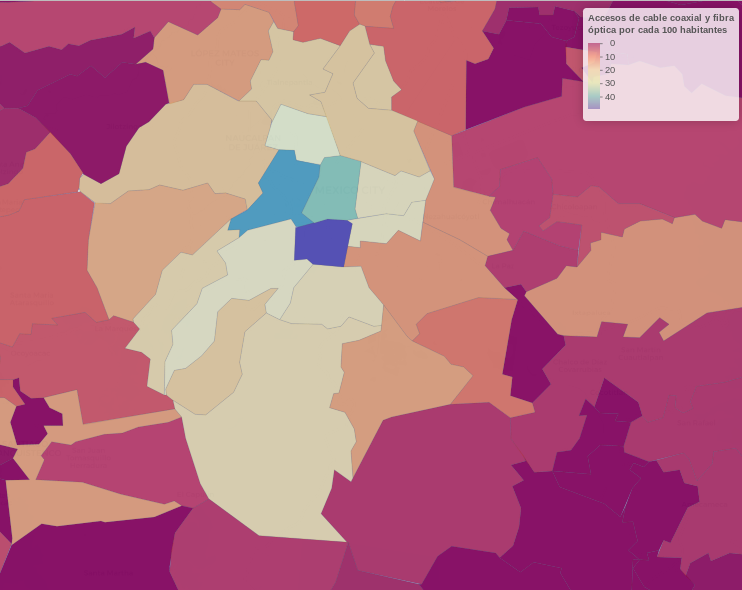
\includegraphics[width=0.5\linewidth]{images/pen_habs_cdmx.png}
\caption{Penetración de cable coaxial y fibra alrededor de CDMX}
\label{fig:pen_habs_cdmx}
\end{figure}

\subsection{Hola}

Dado que, como se hizo notar en la sección previa, la cobertura de los municipios es heterogénea, para estudiarla se categorizará a cada municipio del país acuerdo a su nivel de penetración de banda ancha fija, con referencia al valor promedio de los países miembros de la OCDE (30.92 accesos por cada 100 habitantes):
\begin{table}[tbhp]
	\centering
	\caption{Niveles de penetración en un municipio\label{table:clasifpen}}
	\begin{tabular}{@{}ll@{}}
		\toprule
		%\rowcolor[HTML]{EFEFEF} 
		Nivel de penetración & Rango  de penetración            \\ \midrule
		Muy Alta  & $Penetracion > Media \ OCDE$         \\ 
		%\rowcolor[HTML]{EFEFEF} 
		Alta    & $20 < Penetracion \leq Media \ OCDE$ \\ 
		Media    & $10 < Penetracion \leq 20$  \\ 
		%\rowcolor[HTML]{EFEFEF} 
		Baja      & $0 < Penetracion \leq 10$  \\ 
		%\rowcolor[HTML]{EFEFEF} 
		Nula      & $Penetracion =0$            \\ \bottomrule
	\end{tabular}
	%\addtabletext{Clasificación de municipios según su rango de penetración de BAF}
\end{table}

%\section*{Sections: Theory, Methods, Results, Discussion...}

\section{Modelación y niveles de cobertura de banda ancha fija en municipios}

En linea con la exposición anterior, se busca explorar la posibilidad de que la información del entorno socio-económico, demográfico y tecnológico de los municipios sirva como una vía que permita inferir el nivel de cobertura actual de los servicios de banda ancha fija que los operadores hayan desplegado a la fecha.



\subsection*{Selección de variables relevantes}

Uso de matriz de correlaciones

Uso de regresión de Lasso sobre el número bruto de la penetración.

Variables que se añadieron (densidad de hogares, densidad poblacional)

\subsection{Modelo de regresión logística para clasificación}

Pendiente: desarrollo

\subsection{Bosques aleatorios para problemas de clasificación}

Consideremos ${\mathcal D} =\{(x^{(i)}, y^{(i)})\}_{i=1}^n$ una colección de puntos de entrenamiento junto con sus respectivas etiquetas, para los cuales se construye una colección de muestras bootstrap ${\mathcal D}_1^*, {\mathcal D}_2^*, \ldots, {\mathcal D}_B^*$ y se fija un número $m$ que permitirá seleccionar un subconjunto de sus características.

Para cada unas de esta muestras bootstrap construimos un árbol, bajo el siguiente esquema: a)
En cada nodo candidato a particionar, escogemos al azar $m$ variables de las disponibles; 2) Buscamos la mejor variable y punto de corte (como en un árbol normal) pero solo entre las variables que seleccionamos al azar, 3) Seguimos hasta construir un árbol grande.

Al consolidar un conjunto de 

$T^*(x) = argmax_g \{ \# \{i|T_b^*(x)=g\}\}.$

Bosques aleatorios pueden ayudar a reducir el error de predicción gracias a una reducción a veces considerable de varianza. El objetivo final es reducir la varianza alta que producen árboles normales debido a la forma tan agresiva de construir sus cortes.

Pendiente: desarrollo

\subsection{Extra Gradient boosting (XGboost) para problemas de clasificación) }
Los métodos basados en ensambles de árboles parten de la idea de que al combinar cierta cantidad de modelos predictores débiles para un problema. Esto se traduce en aplicar un proceso recursivo de aprendizaje

\begin{equation}
\hat{y}_i = \sum_{k=1}^K f_k(x_i), f_k \in \mathcal{F}
\end{equation}



En el contexto de 

Esta técnica se basa en un aprendizaje de funcione
Start from constant prediction, add a new function each time


Pendiente: desarrollo

\section{Figures and Tables}

Figures and Tables should be labeled and referenced in the standard way using the \verb|\label{}| and \verb|\ref{}| commands.


%\begin{figure}[tbhp]
%\centering
%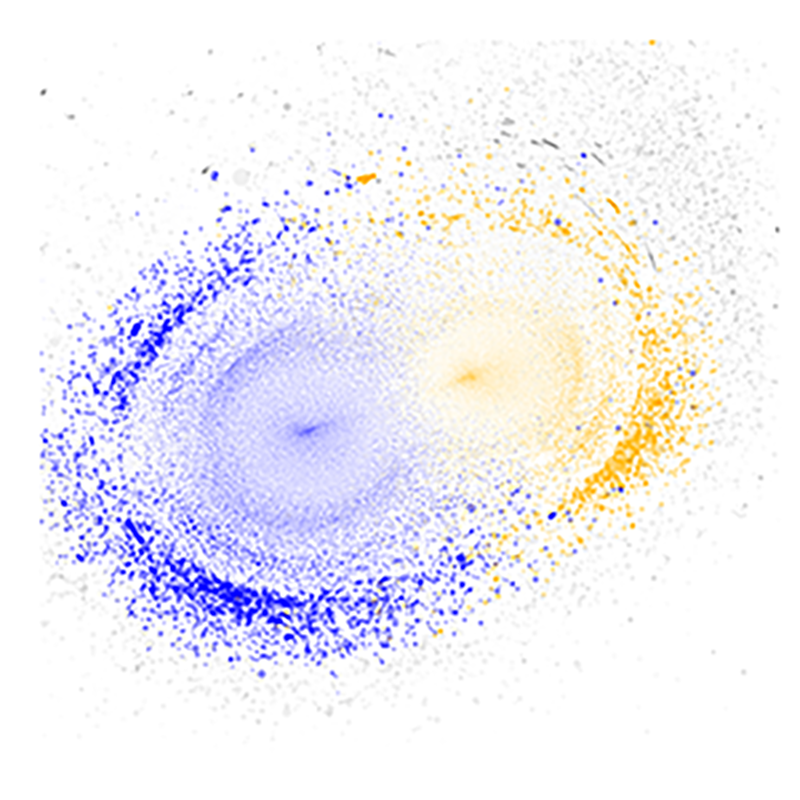
\includegraphics[width=.8\linewidth]{net_red}
%\caption{Placeholder image of a Network with a long example caption to show justification setting.}
%\label{fig:net}
%\end{figure}


%Figure \ref{fig:net} shows an example of how to insert a column-wide figure. To insert a figure wider than one column, please use the \verb|\begin{figure*}...\end{figure*}| environment. Figures wider than one column should be sized to 11.4 cm or 17.8 cm wide. Use \verb|\begin{SCfigure*}...\end{SCfigure*}| for a wide figure with side captions.



%
%
%\begin{table}%[tbhp]
%	%\centering
%	\caption{Character Level Combat Outcomes\label{table:char_main}}
%	\begin{tabular}{@{\extracolsep{5pt}}lccc} 
%		\\[-1.8ex]\hline 
%		\hline \\[-1.8ex] 
%		& \multicolumn{3}{c}{\textit{Dependent variable:}} \\ 
%		\cline{2-4} 
%		\\[-1.8ex] & Combat & Combat & Combat\\ 
%		\\[-1.8ex] & Amount & Variability & Skill \\ 
%		\\[-1.8ex] & (1) & (2) & (3)\\ 
%		\hline \\[-1.8ex] 
%		Man - Male & 0.042$^{***}$ & 5.659$^{***}$ & 0.031$^{***}$  \\ 
%		& (0.002) & (0.056) & (0.0004)  \\ 
%		Woman - Female & $-$0.026$^{***}$ & 1.529$^{***}$ & 0.011$^{***}$  \\ 
%		& (0.005) & (0.143) & (0.001)  \\ 
%		Woman - Male & 0.010 & 0.375 & 0.005$^{*}$  \\ 
%		& (0.009) & (0.272) & (0.002)  \\ 
%		Player Age & $-$0.077$^{***}$ &  &  $-$0.003$^{***}$\\ 
%		& (0.001) &  & (0.0002) \\ 
%		Mil. Label & 0.135$^{***}$ &  & 0.060$^{***}$ \\ 
%		& (0.002) &  & (0.0004) \\ 
%		Constant &  & $-$97.425$^{***}$ &   \\ 
%		&  & (0.046) &   \\ 
%		\hline 
%		Char. Order FEs     &       Y&       N&     Y\\
%		Create Date FEs     &       Y&       N&     Y\\
%		\hline  
%		Observations & 576,430 & 576,430 & 576,430 \\ 
%		R$^{2}$ & 0.028 & 0.018 & 0.089  \\ 
%		\hline 
%	\end{tabular} 
%	\vspace{1mm}
%	\addtabletext{*  p$<$0.05, ** p$<$0.01, *** p$<$0.001 \\
%		This table reports coefficients and standards errors from ordinary least squares regressions. In all models we can reject the null that \emph{Woman - Female} and \emph{Woman - Male} are equivalent with p $<$ .01. In models 2 and 3 we can reject the null that the gender gaps within sex are equivalent ((\emph{Woman - Male}) - (\emph{Woman - Female}) = \emph{Man - Male}) with p $<$ .001.}
%\end{table}


%\texttt{\subsection*{Tables}
%In addition to including your tables within this manuscript file, PNAS requires that each table be uploaded to the submission separately as a “Table” file.  Please ensure that each table .tex file contains a preamble, the \verb|\begin{document}| command, and the \verb|\end{document}| command. This is necessary so that the submission system can convert each file to PDF.
%
%\subsection*{Equations}
%
%Authors may use 1- or 2-column equations in their article, according to their preference.
%
%To allow an equation to span both columns, use the \verb|\begin{figure*}...\end{figure*}| environment mentioned above for figures. Using only \verb|\begin{figure*}...\end{figure*}| keeps the equation in a two collum format
%
%
%\begin{figure}[bt!]
%\begin{align*}
%(x+y)^3&=(x+y)(x+y)^2\\
%       &=(x+y)(x^2+2xy+y^2) \numberthis \label{eqn:example} \\
%       &=x^3+3x^2y+3xy^3+x^3. 
%\end{align*}
%\end{figure}}
%
%
%\section*{References}
%
%References should be cited in alphabethical order; this will be done automatically via bibtex. All references should be included in the main manuscript file.  
%
%
%\acknow{Please include your acknowledgments here, set in a single paragraph. Please do not include any acknowledgments in the Supporting Information, or anywhere else in the manuscript.}

\showacknow{} % Display the acknowledgments section

% Bibliography

\bibliography{ilcss-sample}

\end{document}